\documentclass[10pt,a4paper]{article}
\usepackage{amsmath,amssymb,amsthm,graphicx}
\usepackage[no-math]{fontspec}
\newenvironment{authorclaim}[1]{\par\medskip\noindent\textbf{#1.}\ }{\par\medskip}
\allowdisplaybreaks
\usepackage{graphicx}
\title{Search-to-decision reduction for exponent-p class-two matrix-group isomorphism}
\author{Joshua A. Grochow, Youming Qiao}
\date{doi:10.4230/LIPIcs.CCC.2021.16; CC BY 4.0}
\begin{document}
\maketitle
\noindent\textit{Editorial scope.} Counted once: group search-to-decision Theorem A with its full A-prime tensor mechanism. Both runtime branches and every local support proof included; no separate count for gadgets, dynamic programming or direct applications. Preserves odd prime, class-two/exponent-p matrix-group model, finite-field isometry conventions and oracle bounds.\par\medskip
\noindent\textit{Allowed standard prerequisites (editorial).}\begin{itemize}
\item Finite-field linear algebra, standard permutation-group computations and imported FGS tensor gadget. Original definitions, complete monomial gadget and complete local search/dynamic-programming proofs retained. Separately cited [28] and [32] FGS background is retained with exact reference to Proposition 3.3. Complete source-local constructive Baer proof retained; full 74-item published bibliography.
\end{itemize}\medskip
% Faithful formal-publication context for search/count reductions: Sections1.2 and2.
\section*{Author notation and isometry models}
\paragraph{Vector spaces.} Let $\mathbb F$ be a field. In this paper we only consider finite-dimensional vector spaces over $\mathbb F$. We use $\mathbb F^n$ to denote the vector space of length-$n$ column vectors. The $i$th standard basis vector of $\mathbb F^n$ is denoted $\vec e_i$. Depending on the context, 0 may denote the zero vector space, a zero vector, or an all-zero matrix. For $S$ a set of vectors, we use $\langle S\rangle$ to denote the subspace spanned by elements in $S$.
\paragraph{Some groups.} The general linear group of degree $n$ over a field $\mathbb F$ is denoted by $\mathrm{GL}(n,\mathbb F)$. The symmetric group of degree $n$ is denoted by $S_n$. The natural embedding of $S_n$ into $\mathrm{GL}(n,\mathbb F)$ is to represent permutations by permutation matrices. The subgroup of $\mathrm{GL}(n,\mathbb F)$ consisting of diagonal matrices is called the diagonal subgroup, denoted by $\operatorname{diag}(n,\mathbb F)$. A monomial matrix is a product of a diagonal and a permutation matrix; equivalently, each row and each column has exactly one non-zero entry. The collection of monomial matrices forms a subgroup of $\mathrm{GL}(n,\mathbb F)$, which we call the monomial subgroup and denote by $\operatorname{Mon}(n,\mathbb F)$. It is the semi-direct product $\operatorname{diag}(n,\mathbb F)\rtimes S_n\cong(\mathbb F^*)^n\rtimes S_n$.
\paragraph{Matrices.} Let $\mathrm M(\ell\times n,\mathbb F)$ be the linear space of $\ell\times n$ matrices over $\mathbb F$, and $\mathrm M(n,\mathbb F):=\mathrm M(n\times n,\mathbb F)$. Given $A\in\mathrm M(\ell\times n,\mathbb F)$, $A^t$ denotes the transpose of $A$.
A matrix $A\in\mathrm M(n,\mathbb F)$ is alternating, if for any $u\in\mathbb F^n$, $u^tAu=0$. That is, $A$ represents an alternating bilinear form. Note that in characteristic $\ne2$, alternating is the same as skew-symmetric, but in characteristic 2 they differ (in characteristic 2, skew-symmetric=symmetric). The linear space of $n\times n$ alternating matrices over $\mathbb F$ is denoted by $\Lambda(n,\mathbb F)$.
The $n\times n$ identity matrix is denoted by $I_n$, and when $n$ is clear from the context, we may just write $I$. The elementary matrix $E_{i,j}$ is the matrix with the $(i,j)$th entry being 1, and other entries being 0. The $(i,j)$-th elementary alternating matrix is the matrix $E_{i,j}-E_{j,i}$.
\paragraph{Matrix tuples.} We use $\mathrm M(\ell\times n,\mathbb F)^m$ to denote the linear space of $m$-tuples of $\ell\times n$ matrices. Boldface letters like $\mathbf A$ and $\mathbf B$ denote matrix tuples. Let $\mathbf A=(A_1,\ldots,A_m)$, $\mathbf B=(B_1,\ldots,B_m)\in\mathrm M(\ell\times n,\mathbb F)^m$. Given $P\in\mathrm M(\ell,\mathbb F)$ and $Q\in\mathrm M(n,\mathbb F)$, $P\mathbf A Q:=(PA_1Q,\ldots,PA_mQ)\in\mathrm M(\ell,\mathbb F)$. Given $R=(r_{i,j})_{i,j\in[m]}\in\mathrm M(m,\mathbb F)$, $\mathbf A^R:=(A'_1,\ldots,A'_m)\in\mathrm M(m,\mathbb F)$ where $A'_i=\sum_{j\in[m]}r_{j,i}A_j$.
\begin{authorclaim}{Remark5}
In particular, note that the coefficients in the formula of defining $A'_i$ correspond to the entries in the $i$th column of $R$. While this choice is immaterial (we could have chosen the opposite convention), all of our later calculations are consistent with this convention.
\end{authorclaim}
Given $\mathbf A,\mathbf B\in\mathrm M(\ell\times n,\mathbb F)^m$, we say that $\mathbf A$ and $\mathbf B$ are isometric, if there exists $P\in\mathrm{GL}(n,\mathbb F)$, such that $P^t\mathbf A P=\mathbf B$. Finally, $\mathbf A$ and $\mathbf B$ are pseudo-isometric if there exist $P\in\mathrm{GL}(n,\mathbb F)$ and $R\in\mathrm{GL}(m,\mathbb F)$, such that $P^t\mathbf A P=\mathbf B^R$.
\paragraph{Matrix spaces.} Linear subspaces of $\mathrm M(\ell\times n,\mathbb F)$ are called matrix spaces. Calligraphic letters like $\mathcal A$ and $\mathcal B$ denote matrix spaces. By a slight abuse of notation, for $\mathbf A\in\mathrm M(\ell\times n,\mathbb F)^m$, we use $\langle\mathbf A\rangle$ to denote the subspace spanned by those matrices in $\mathbf A$. For $\mathbf A,\mathbf B\in\mathrm M(n,\mathbb F)^m$, we say that the spaces $\langle\mathbf A\rangle,\langle\mathbf B\rangle$ are isometric iff the tuples $\mathbf A,\mathbf B$ are pseudo-isometric.
\begin{authorclaim}{Definition4 (The Alternating Matrix Space Isometry problem)}
Input: $A_1,\ldots,A_m$ and $B_1,\ldots,B_m$, $n\times n$ alternating matrices over a field $\mathbb F$.
Decide: Is there a $L\in\mathrm{GL}(n,\mathbb F)$, such that the linear span of $\{A_i:i\in[m]\}$ is equal to the linear span of $\{L^tB_iL:i\in[m]\}$?
\end{authorclaim}
\paragraph{3-way arrays.} Let $\mathrm T(\ell\times n\times m,\mathbb F)$ be the linear space of $\ell\times n\times m$ 3-way arrays over $\mathbb F$. We use the fixed-width teletypefont for 3-way arrays, like $\mathtt A,\mathtt B$, etc..
Given $\mathtt A\in\mathrm T(\ell\times n\times m,\mathbb F)$, we can think of $\mathtt A$ as a 3-dimensional table, where the $(i,j,k)$th entry is denoted as $\mathtt A(i,j,k)\in\mathbb F$. We can slice $\mathtt A$ along one direction and obtain several matrices, which are then called slices. For example, slicing along the first coordinate, we obtain the horizontal slices, namely $\ell$ matrices $A_1,\ldots,A_\ell\in\mathrm M(n\times m,\mathbb F)$, where $A_i(j,k)=\mathtt A(i,j,k)$. Similarly, we also obtain the lateral slices by slicing along the second coordinate, and the frontal slices by slicing along the third coordinate.
We will often represent a 3-way array as a matrix whose entries are vectors. That is, given $\mathtt A\in\mathrm T(\ell\times n\times m,\mathbb F)$, we can write
\[\mathtt A=\begin{bmatrix}w_{1,1}&w_{1,2}&\cdots&w_{1,n}\\w_{2,1}&w_{2,2}&\cdots&w_{2,n}\\\vdots&\vdots&\ddots&\vdots\\w_{\ell,1}&w_{\ell,2}&\cdots&w_{\ell,n}\end{bmatrix},\]
where $w_{i,j}\in\mathbb F^m$, so that $w_{i,j}(k)=\mathtt A(i,j,k)$. Note that, while $w_{i,j}\in\mathbb F^m$ are column vectors, in the above representation of $\mathtt A$, we should think of them as along the direction ``orthogonal to the paper.'' Following [45], we call $w_{i,j}$ the tube fibers of $\mathtt A$. Similarly, we can have the row fibers $v_{i,k}\in\mathbb F^n$ such that $v_{i,k}(j)=\mathtt A(i,j,k)$, and the column fibers $u_{j,k}\in\mathbb F^\ell$ such that $u_{j,k}(i)=\mathtt A(i,j,k)$.
Given $P\in\mathrm M(\ell,\mathbb F)$ and $Q\in\mathrm M(n,\mathbb F)$, let $P\mathtt A Q$ be the $\ell\times n\times m$ 3-way array whose $k$th frontal slice is $PA_kQ$. For $R=(r_{i,j})\in\mathrm{GL}(m,\mathbb F)$, let $\mathtt A^R$ be the $\ell\times n\times m$ 3-way array whose $k$th frontal slice is $\sum_{k'\in[m]}r_{k',k}A_{k'}$. Note that these notations are consistent with the notations for matrix tuples above, when we consider the matrix tuple $\mathbf A=(A_1,\ldots,A_k)$ of frontal slices of $\mathtt A$.

\begin{authorclaim}{TheoremA}
Let $p$ be an odd prime, and let $\operatorname{GpIso2Exp}(p)$ denote the isomorphism problem for $p$-groups of class 2 and exponent $p$ in the model of matrix groups over $\mathbb F_p$. For groups of order $p^n$, there is a search-to-decision reduction for $\operatorname{GpIso2Exp}(p)$ running in time $p^{O(n)}=\operatorname{poly}(|G|)$.
\end{authorclaim}

% Faithful formal-publication transcription of Section4.1, Lemma8 and entire proof. Published graphical arrays are preserved as vector crops.
\section*{4 Search-to-decision reduction by restricting to monomial groups}
\subsection*{4.1 The gadget restricting to the monomial group}
In this section, we present the gadget that restricts to the monomial group in the setting of Alternating Matrix Space Isometry. To show this, we will need the concept of monomial isometry; see Some Groups above. Recall that a matrix is monomial if, equivalently, it can be written as $DP$ where $D$ is a nonsingular diagonal matrix and $P$ is a permutation matrix. We say two matrix spaces $\mathcal A,\mathcal B$ are monomially isometric if there is some $M\in\operatorname{Mon}(n,\mathbb F)$ such that $M^t\mathcal A M=\mathcal B$.
\begin{authorclaim}{Lemma8}
Alternating Matrix Space Monomial Isometry reduces to Alternating Matrix Space Isometry. More specifically, there is a $\operatorname{poly}(n,m)$-time algorithm $r$ taking alternating matrix tuples to alternating matrix tuples, such that for $\mathbf A,\mathbf B\in\Lambda(n,\mathbb F)^m$, the matrix spaces $\mathcal A=\langle\mathbf A\rangle$ and $\mathcal B=\langle\mathbf B\rangle$ are monomially isometric if and only if the matrix spaces $\langle r(\mathbf A)\rangle$ and $\langle r(\mathbf B)\rangle$ are isometric.
\end{authorclaim}
The gadget used in Lemma8 is essentially to apply the gadget in Proposition7 ``in two directions.'' Still, to prove the correctness requires some work.
\begin{proof}
For $\mathbf A=(A_1,\ldots,A_m)\in\Lambda(n,\mathbb F)^m$, define $r(\mathbf A)$ to be the alternating matrix tuple $\widetilde{\mathbf A}=(\widetilde A_1,\ldots,\widetilde A_{m+n^2})\in\Lambda(n+n^2,\mathbb F)^{m+n^2}$, where
\begin{enumerate}
\item For $k=1,\ldots,m$, $\widetilde A_k=\begin{bmatrix}A_k&0\\0&0\end{bmatrix}$.
\item For $k=m+(i-1)n+j$, $i\in[n],j\in[n]$, $\widetilde A_k$ is the elementary alternating matrix $E_{i,in+j}-E_{in+j,i}$.
\end{enumerate}
At this point, some readers may wish to look at the large matrix in Equation2 and/or at Figure2.
It is clear that $r$ can be computed in time $\widetilde O((m+n^2)(n^2+n))=\operatorname{poly}(n,m)$. Given alternating matrix tuples $\mathbf A,\mathbf B$, let $\mathcal A,\mathcal B$ be the corresponding matrix spaces they span, and let $\widetilde{\mathcal A}=\langle r(\mathbf A)\rangle$ and $\widetilde{\mathcal B}=\langle r(\mathbf B)\rangle$. We claim that $\mathcal A$ and $\mathcal B$ are monomially isometric if and only if $\widetilde{\mathcal A}$ and $\widetilde{\mathcal B}$ are isometric.
To prove this, it will help to think of our matrix tuples $\mathbf A,\widetilde{\mathbf A}$, etc. as (corresponding to) 3-way arrays, and to view these 3-way arrays from two different directions. Towards this end, write the 3-way array corresponding to $\mathbf A$ as
\[\mathtt A=\begin{bmatrix}0&a_{1,2}&a_{1,3}&\cdots&a_{1,n}\\-a_{1,2}&0&a_{2,3}&\cdots&a_{2,n}\\-a_{1,3}&-a_{2,3}&0&\cdots&a_{3,n}\\\vdots&\vdots&\vdots&\ddots&\vdots\\-a_{1,n}&-a_{2,n}&-a_{3,n}&\cdots&0\end{bmatrix},\]
where $a_{i,j}$ are vectors in $\mathbb F^m$ (``coming out of the page''), namely $a_{i,j}(k)=A_k(i,j)$. The frontal slices of this array are precisely the matrices $A_1,\ldots,A_m$.
The 3-way array corresponding to $\widetilde{\mathbf A}=r(\mathbf A)$ is then the $(n+1)n\times(n+1)n\times(m+n^2)$ array:
\begin{center}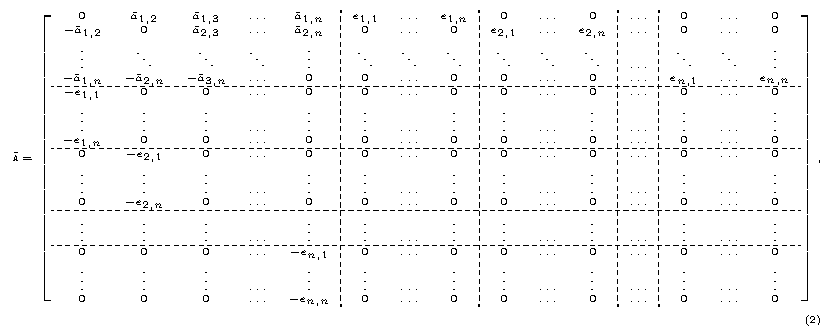
\includegraphics[width=.98\linewidth]{sources/equation2.pdf}\end{center}
where $\widetilde a_{i,j}=\begin{bmatrix}a_{i,j}\\0\end{bmatrix}\in\mathbb F^{m+n^2}$ (here think of the vector $a_{i,j}$ as a column vector, not coming out of the page; in the above array we then lay the column vector $\widetilde a_{i,j}$ ``on its side'' so that it is coming out of the page), and $e_{i,j}:=e_{m+(i-1)n+j}\in\mathbb F^{m+n^2}$, which we can equivalently write as $\begin{bmatrix}0^m\\e_i\otimes e_j\end{bmatrix}$, where we think of $e_i\otimes e_j$ here as a vector of length $n^2$. Note that all the the nonzero blocks besides upper-left ``$\mathtt A$'' block only have nonzero entries that are strictly behind the nonzero entries in the upper-left block.
\begin{center}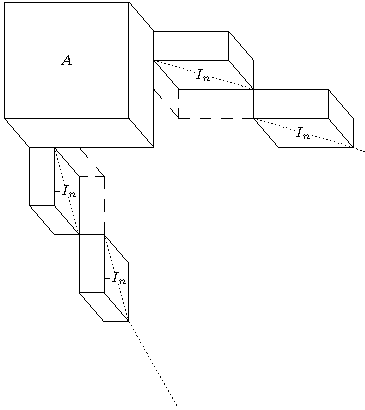
\includegraphics[width=.5\linewidth]{sources/figure2.pdf}\end{center}
\noindent Figure2. Pictorial representation of the reduction for Lemma8.
The second viewpoint, which we will also use below, is to consider the lateral slices of $\widetilde{\mathtt A}$, or equivalently, to view $\widetilde{\mathtt A}$ from the side. When viewing $\widetilde{\mathtt A}$ from the side, we see the $(n+1)n\times(m+n^2)\times(n+1)n$ 3-way array:
\begin{center}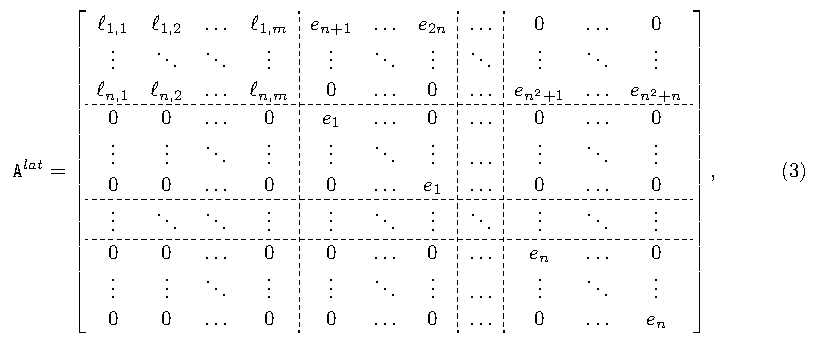
\includegraphics[width=.98\linewidth]{sources/equation3.pdf}\end{center}
where every $\ell_{i,k}\in\mathbb F^{n^2+n}$ has only the first $n$ components being possibly non-zero, namely, $\ell_{i,k}(j)=A_k(i,j)$ for $i\in[n],j\in[n],k\in[m]$ and $\ell_{i,k}(j)=0$ for any $j>n$.
\paragraph{For the only if direction.}
Suppose there exist $P\in\operatorname{Mon}(n,\mathbb F)$ and $Q\in\mathrm{GL}(m,\mathbb F)$, such that $P^t\mathbf A P=\mathbf B^Q$. We can construct $\widetilde P\in\operatorname{Mon}(n+n^2,\mathbb F)$ and $\widetilde Q\in\mathrm{GL}(m+n^2,\mathbb F)$ such that $\widetilde P^t\widetilde{\mathbf A}\widetilde P=\widetilde{\mathbf B}^{\widetilde Q}$. In fact, we will show that we can take $\widetilde P=\begin{bmatrix}P&0\\0&P'\end{bmatrix}$ where $P'\in\operatorname{Mon}(n^2,\mathbb F)$, and $\widetilde Q=\begin{bmatrix}Q&0\\0&Q'\end{bmatrix}$ where $Q'\in\operatorname{Mon}(n^2,\mathbb F)$. It is not hard to see that this form already ensures that the first $m$ matrices in the vector $\widetilde P^t\widetilde{\mathbf A}\widetilde P$ and those of $\widetilde{\mathbf B}^{\widetilde Q}$ are the same, since when $\widetilde P,\widetilde Q$ are of this form, those first $m$ matrices are controlled entirely by the $P$ (resp., $Q$) in the upper-left block of $\widetilde P$ (resp., $\widetilde Q$).
The remaining question is then how to design appropriate $P'$ and $Q'$ to take care of the last $n^2$ matrices in these tuples. This actually boils down to applying the following simple identity, but ``in 3 dimensions:'' Let $P$ be the permutation matrix corresponding to $\sigma\in S_n$, so that $Pe_i=e_{\sigma(i)}$, and $e_i^tP=e_{\sigma^{-1}(i)}^t$. Let $D=\operatorname{diag}(\alpha_1,\ldots,\alpha_n)$ be a diagonal matrix. Then
\begin{equation}\tag{4}P^tDP=\operatorname{diag}(\alpha_{\sigma^{-1}(1)},\ldots,\alpha_{\sigma^{-1}(n)}).\end{equation}
To see how Equation4 helps in our setting, it is easier to focus attention on the lower right $n^2\times n^2$ sub-array of $\mathtt A^{\mathrm{lat}}$, which can be represented as a symbolic matrix
\[M=\begin{bmatrix}x_1I_n&0&\cdots&0\\0&x_2I_n&\cdots&0\\\vdots&\vdots&\ddots&\vdots\\0&0&\cdots&x_nI_n\end{bmatrix}.\]
Here we think of the $x_i$'s as independent variables, whose indices correspond to ``how far into the page'' they are. That is, $x_i$ corresponds to the vector $\vec e_i$ in $\mathtt A^{\mathrm{lat}}$, which is coming out of the page and has its only nonzero entry $i$ slices back from the page.
Then the action of $P$ permutes the $x_i$'s and multiplies them by some scalars, the action of $P'$ is on the left-hand side, and the action of $Q'$ is on the right-hand side. Let $\sigma$ be the permutation supporting $P$. Then $P$ sends $M$ to
\[M^P=\begin{bmatrix}\alpha_{\sigma(1)}x_{\sigma(1)}I_n&0&\cdots&0\\0&\alpha_{\sigma(2)}x_{\sigma(2)}I_n&\cdots&0\\\vdots&\vdots&\ddots&\vdots\\0&0&\cdots&\alpha_{\sigma(n)}x_{\sigma(n)}I_n\end{bmatrix}.\]
So setting $P'=\sigma\otimes I_n$, $Q'$ the monomial matrix supported by $\sigma\otimes I_n$ with scalars being $1/\alpha_i$'s, we have $P'^tM^PQ'=M$ by Equation4.
\paragraph{For the if direction.}
Suppose there exist $\widetilde P\in\mathrm{GL}(n+n^2,\mathbb F)$ and $\widetilde Q\in\mathrm{GL}(m+n^2,\mathbb F)$, such that $\widetilde P^t\widetilde{\mathbf A}\widetilde P=\widetilde{\mathbf B}^{\widetilde Q}$. The key feature of these gadgets now comes into play: consider the lateral slices of $\widetilde{\mathtt A}$, which are the frontal slices of $\mathtt A^{\mathrm{lat}}$ (which may be easier to visualize by looking at Equation3 and Figure2). The first $n$ lateral slices of $\widetilde{\mathtt A}$ and $\widetilde{\mathtt B}$ are of rank $\ge n$ and $<2n$, while the other lateral slices are of rank $<n$ (in fact, they are of rank 1; note that without loss of generality we may assume $n>1$, for the only $1\times1$ alternating matrix space is the zero space). Furthermore, left multiplying a lateral slice by $\widetilde P^t$ and right multiplying it by $\widetilde Q$ does not change its rank. However, the action of $\widetilde P$ here is by $\widetilde P^t\widetilde{\mathbf A}\widetilde P$, and while the $\widetilde P^t$ here corresponds to left multiplication on the lateral slices (=frontal slices of $\mathtt A^{\mathrm{lat}}$), the $\widetilde P$ on the right here corresponds to taking linear combinations of the lateral slices. In other words, just as $\mathtt A^{\mathrm{lat}}$ is the ``side view'' of $\widetilde{\mathtt A}$, $(\widetilde P^t\mathtt A^{\mathrm{lat}}\widetilde Q)^{\widetilde P}$ is the side view of $(\widetilde P^t\widetilde{\mathtt A}\widetilde P)^{\widetilde Q}$. Taking linear combinations of the lateral slices could, in principle, alter their rank; we will use the latter possibility to show that $\widetilde P$ must be of a constrained form.
Write $\widetilde P=\begin{bmatrix}P_{1,1}&P_{1,2}\\P_{2,1}&P_{2,2}\end{bmatrix}$ where $P_{1,1}$ is of size $n\times n$. We first claim that $P_{1,2}=0$. For if not, then in $(\mathtt A^{\mathrm{lat}})^{\widetilde P}$ (the side view), one of the last $n^2$ frontal slices receives a nonzero contribution from one of the first $n$ frontal slices of $\mathtt A^{\mathrm{lat}}$. Looking at the form of these slices from Equation3, we see that any such nonzero combination will have rank $\ge n$, but this is a contradiction since the corresponding slice in $\mathtt B^{\mathrm{lat}}$ has rank 1. Thus $P_{1,2}=0$, and therefore $P_{1,1}$ must be invertible, since $\widetilde P$ is.
Finally, we claim that $P_{1,1}$ has to be a monomial matrix. If not, then some frontal slice of $(\mathtt A^{\mathrm{lat}})^{\widetilde P}$ among the first $n$ would have a contribution from more than one of these $n$ slices. Considering the lower-right $n^2\times n^2$ sub-matrix of such a slice, we see that it would have rank exactly $kn$ for some $k\ge2$, which is again a contradiction since the first $n$ slices of $\mathtt B^{\mathrm{lat}}$ all have rank $<2n$. It follows that $P_{1,1}^tA_iP_{1,1}$, $i\in[m]$, are in $\mathcal B$, and thus $\mathcal A$ and $\mathcal B$ are monomially isometric via $P_{1,1}$.
\end{proof}

\begin{authorclaim}{TheoremA'}
Given an oracle deciding Alternating Matrix Space Isometry, the task of finding an isometry between two alternating matrix spaces $\mathcal A,\mathcal B\in\Lambda(n,\mathbb F_q)$, if it exists, can be solved using at most $q^{O(n)}$ oracle queries each of size at most $O(n^2)$, and in time either $q^{O(n)}\cdot n!=q^{\widetilde O(n)}$, or $q^{O(n+m)}$.
\end{authorclaim}

\begin{proof}
We first present the gadget construction. Then based on this gadget, we present the search-to-decision reduction.
\paragraph{Gadget construction.} Let $\mathbf A=(A_1,\ldots,A_m)$ be an ordered linear basis of $\mathcal A$, and let $\mathtt A\in\mathrm T(n\times n\times m,\mathbb F_q)$ be the 3-way array constructed from $\mathbf A$, so we can write
\[\mathtt A=\begin{bmatrix}0&a_{1,2}&a_{1,3}&\cdots&a_{1,n}\\-a_{1,2}&0&a_{2,3}&\cdots&a_{2,n}\\-a_{1,3}&-a_{2,3}&0&\cdots&a_{3,n}\\\vdots&\vdots&\vdots&\ddots&\vdots\\-a_{1,n}&-a_{2,n}&-a_{3,n}&\cdots&0\end{bmatrix},\]
where $a_{i,j}\in\mathbb F^m$, $1\le i<j\le n$ thought of as a vector coming out of the page.
We first consider a 3-tensor $\widetilde{\mathtt A}_i$ constructed from $\mathtt A$, for any $1\le i\le n-1$, as $\widetilde{\mathtt A}_i=$
\begin{center}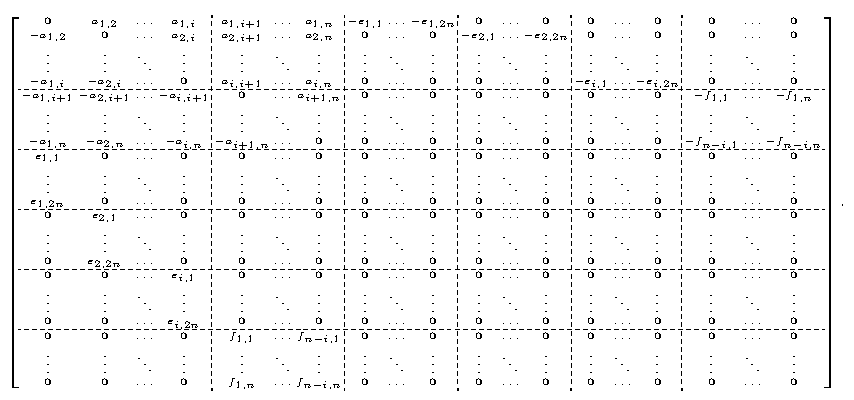
\includegraphics[width=.98\linewidth]{sources/search-gadget.pdf}\end{center}
where $e_{j,k}$ is the $(m+2n(j-1)+k)$th standard basis vector, and $f_{j,k}$ is the $(m+2ni+n(j-1)+k)$th standard basis vector. A pictorial description can be seen by combining Figure2 (for the $e_{j,k}$) and [32, Figure3] (for the $f_{j,k}$).
We claim the following.
\begin{authorclaim}{Claim10}
If there exist invertible matrices $P$ and $Q$ to satisfy $P^t\widetilde{\mathtt A}_iP=\widetilde{\mathtt B}_i^Q$, then $P$ must be in the form $\begin{bmatrix}P_{1,1}&0&0\\0&P_{2,2}&0\\P_{3,1}&P_{3,2}&P_{3,3}\end{bmatrix}$, where $P_{1,1}$ is a monomial matrix of size $i\times i$, $P_{2,2}$ is of size $(n-i)\times(n-i)$, and $P_{3,3}$ is of size $(2ni+n)\times(2ni+n)$.
Furthermore, there exist such $P$ and $Q$ if and only if $\mathcal A$ and $\mathcal B$ are isometric by a matrix of the form $\begin{bmatrix}P_{1,1}&0\\0&P_{2,2}\end{bmatrix}$ where $P_{1,1}$ is a monomial matrix of size $i\times i$.
\end{authorclaim}
\begin{proof}
This claim is immediate by combining the arguments for the FGS gadget [28] as used in [32], and the monomial-restricting gadget introduced in Section4.1. We only outline the argument and point out some subtle issues here.
First, observe that for the lateral slices of $\widetilde{\mathtt A}_i$:
\begin{itemize}
\item The first $i$ lateral slices have rank in $[2n,3n)$. Note that the rank is strictly less than $3n$ because some tube fibers (coming out of the page) are 0 in the upper-left $n\times n$ sub-array.
\item The next $n-i$ lateral slices have rank in $[n,2n)$.
\item The remaining $2ni+n$ lateral slices have rank in $[1,n)$ (since $i\ge1$.)
\end{itemize}
Because of the above, for $P$ and $Q$ to satisfy $P^t\widetilde{\mathtt A}_iP=\widetilde{\mathtt B}_i^Q$, $P$ must be in the required form.
It is the furthermore statement that requires certain care. The only if direction is straightforward: after observing that $P$ has to be of the above form, we can easily verify that $\begin{bmatrix}P_{1,1}&0\\0&P_{2,2}\end{bmatrix}$ is an isometry from $\mathcal A$ to $\mathcal B$. For the if direction, starting from $\begin{bmatrix}P_{1,1}&0\\0&P_{2,2}\end{bmatrix}$ and $Q_{1,1}\in\mathrm{GL}(m,\mathbb F)$, we need to design $P_{3,3}\in\mathrm{GL}(2ni+n,\mathbb F)$ and $Q_{2,2}\in\mathrm{GL}(2ni+n(n-i),\mathbb F)$ such that letting
\[P=\begin{bmatrix}P_{1,1}&0&0\\0&P_{2,2}&0\\0&0&P_{3,3}\end{bmatrix}\quad\text{and}\quad Q=\begin{bmatrix}Q_{1,1}&0\\0&Q_{2,2}\end{bmatrix},\]
we have $P^t\widetilde{\mathtt A}_iP=\widetilde{\mathtt B}_i^Q$. This can be achieved by combining the arguments for the only if directions in the proofs of Lemma8 and [32, Proposition3.3].
\end{proof}
\paragraph{The search-to-decision reduction.} Given these preparations, we now present the search-to-decision reduction for Alternating Matrix Space Isometry. Recall that this requires us to use the decision oracle $\mathcal O$ to compute an explicit isometry transformation $P\in\mathrm{GL}(n,q)$, if $\mathcal A$ and $\mathcal B$ are indeed isometric. Think of $P$ as sending the standard basis $(\vec e_1,\ldots,\vec e_n)$ to another basis $(v_1,\ldots,v_n)$, where $\vec e_i$ and $v_i$ are in $\mathbb F_q^n$.
In the first step, we guess $v_1$, the image of $\vec e_1$, and a complement subspace of $\langle v_1\rangle$, at the cost of $q^{O(n)}$. For each such guess, let $P_1$ be the matrix which sends $\vec e_1\mapsto v_1$ and sends $\langle\vec e_2,\ldots,\vec e_n\rangle$ to the chosen complementary subspace arbitrarily. We apply $P_1$ to $\mathtt A$, and still call the resulting 3-way array $\mathtt A$ in the following. Then construct $\widetilde{\mathtt A}_1$ and $\widetilde{\mathtt B}_1$, and feed these two instances to the oracle $\mathcal O$. Note that, since $P_{1,1}$ (using notation as above) must be monomial, any equivalence between $\widetilde{\mathtt A}_1$ and $\widetilde{\mathtt B}_1$ must preserve our choice of $v_1$ up to scale. Thus, clearly, if $\mathcal A$ and $\mathcal B$ are indeed isometric and we guess the correct image of $\vec e_1$, then the oracle $\mathcal O$ will return yes (and conversely).
In the second step, we guess $v_2$, the image of $\vec e_2$, and a complement subspace of $\langle v_2\rangle$ within $\langle\vec e_2,\ldots,\vec e_n\rangle$, at the cost of $q^{O(n)}$. Note here that the previous step guarantees that there is an isometry respecting the direct sum decomposition $\langle v_1\rangle\oplus\langle\vec e_2,\ldots,\vec e_n\rangle$, so we need only search for a complement of $v_2$ within $\langle\vec e_2,\ldots,\vec e_n\rangle$, and not a more general complement of $\langle v_1,v_2\rangle$ in all of $\mathbb F_q^n$. This is crucial for the runtime, as at the $n/2$ step, the latter strategy would result in searching through $q^{\Theta(n^2)}$ possibilities.
For each such guess, we apply the corresponding transformation to $\mathtt A$ (and again call the resulting 3-way array $\mathtt A$). Then construct $\widetilde{\mathtt A}_2$ and $\widetilde{\mathtt B}_2$, and feed these two instances to the oracle $\mathcal O$. Clearly, if $\mathcal A$ and $\mathcal B$ are indeed isometric and we guess the correct image of $\vec e_2$ (and $\vec e_1$ from the previous step), then the oracle $\mathcal O$ will return yes. However, there is a small caveat here, namely we may guess some image of $\vec e_2$, such that $\mathcal A$ and $\mathcal B$ are actually isometric by some matrix $P$ of the form $\begin{bmatrix}P_{1,1}&0\\0&P_{2,2}\end{bmatrix}$ where $P_{1,1}$ is a monomial matrix of size 2 (instead of the more desired diagonal matrix). But this is fine, as it still ensures $P_{1,1}$ to be monomial, which is the key property to keep. This means that our choices of $\{v_1,v_2\}$ is correct as a set up to scaling, so we proceed.
In general, in the $i$th step, we maintain the property that $\mathcal A$ and $\mathcal B$ are isometric by some $P=\begin{bmatrix}P_{1,1}&0\\0&P_{2,2}\end{bmatrix}$ where $P_{1,1}$ is a monomial matrix of size $(i-1)\times(i-1)$. We guess $v_i$, the image of $\vec e_i$ in $\langle\vec e_i,\ldots,\vec e_n\rangle$, and a complement subspace of $\langle v_i\rangle$ within $\langle\vec e_i,\ldots,\vec e_n\rangle$. This cost is $q^{O(n)}$. For each such guess, we apply the corresponding transformation to $\mathtt A$ (and call the resulting 3-way array $\mathtt A$). Then construct $\widetilde{\mathtt A}_i$ and $\widetilde{\mathtt B}_i$, and feed these two instances to the oracle $\mathcal O$. Once we guess correctly, we ensure that $\mathcal A$ and $\mathcal B$ are isometric by $P=\begin{bmatrix}P_{1,1}&0\\0&P_{2,2}\end{bmatrix}$ where $P_{1,1}$ is a monomial matrix of size $i\times i$.
So after the $(n-1)$th step, we know that $\mathcal A$ and $\mathcal B$ are isometric by a monomial transformation. As the number of all monomial transformations is $(q-1)^n\cdot n!\le q^n\cdot2^{n\log n}=q^{\widetilde O(n)}$, we can enumerate all monomial transformations and check correspondingly. This gives an algorithm in time $q^{\widetilde O(n)}$. By resorting to Proposition11 which solves Alternating Matrix Space Monomial Isometry in time $q^{O(n+m)}$, we have an algorithm in time $q^{O(n+m)}$.
Note that all the instances we feed into the oracle $\mathcal O$ are of size $O(n^2)$. This concludes the proof.
\end{proof}
\section*{4.3 A simply-exponential algorithm for monomial isometry of alternating matrix spaces}
We now state the algorithm for monomial isometry used in TheoremA'.
\begin{authorclaim}{Proposition11}
Let $\mathcal A,\mathcal B\le\Lambda(n,q)$ be $m$-dimensional. Then there exists a $q^{O(n+m)}$-time algorithm that decides whether $\mathcal A$ and $\mathcal B$ are monomially isometric, and if so, computes an explicit monomial isometry.
\end{authorclaim}
\begin{proof}
Let $\mathcal A,\mathcal B\le\Lambda(n,q)$ be two $m$-dimensional alternating matrix spaces. Clearly, by incurring a multiplicative factor of $q^n$, we can reduce to the problem of testing whether $\mathcal A$ and $\mathcal B$ are permutationally isometric, i.e. whether there exists a permutation matrix $T\in\mathrm{GL}(n,q)$, such that $T^t\mathcal A T=\mathcal B$. We will solve this problem in time $2^{O(n)}\cdot q^{O(m)}$. This would give an algorithm with total running time $q^n\cdot2^{O(n)}\cdot q^{O(m)}=q^{O(n+m)}$. The basic idea of the algorithm comes from Luks's dynamic programming technique for Hypergraph Isomorphism [53].
\paragraph{Reducing to a generalized linear code equivalence problem.} Suppose $\mathcal A=\langle A_1,\ldots,A_m\rangle$, and $\mathcal B=\langle B_1,\ldots,B_m\rangle$. Let $\mathtt A$ and $\mathtt B$ be the $n\times n\times m$ 3-way arrays formed by the given bases of $\mathcal A$ and $\mathcal B$. For $S\subseteq[n]$ of size $s$, let $(A_i)_S$ be the submatrix of $A_i$ with row and column indices in $S$. Then let $\mathtt A_S$ be the $s\times s\times m$ 3-way array formed by $((A_1)_S,\ldots,(A_m)_S)$. Similarly we can define $\mathtt B_S$ for $S\subseteq[n]$.
For each $S\subseteq[n]$ of size $s$, let $\operatorname{Iso}(\mathtt A_{[s]},\mathtt B_S)$ be the coset in $S_n\times\mathrm{GL}(m,q)$, such that $(A,B)\in S_n\times\mathrm{GL}(m,q)$ if and only if the natural action of $(A,B)$ sends $\mathtt A_{[s]}$ to $\mathtt B_S$. Since all the matrices are alternating, their diagonal entries are zero, and thus $\mathtt A_{\{i\}}$ and $\mathtt B_{\{i\}}$ are both the $1\times1\times m$ zero vector for any $i$. It follows that if $s=1$ and $S=\{i\}$, $\operatorname{Iso}(\mathtt A_{[1]},\mathtt B_S)=G\times\mathrm{GL}(m,q)$, where $G$ is the coset of $S_n$ consisting of permutations sending 1 to $i$.
Suppose we have computed $\operatorname{Iso}(\mathtt A_{[s]},\mathtt B_S)$ for all $s<t$. Fix $T\subseteq[n]$, $|T|=t$, and let us compute $\operatorname{Iso}(\mathtt A_{[t]},\mathtt B_T)$. For any $(A,B)\in\operatorname{Iso}(\mathtt A_{[t]},\mathtt B_T)$, $A$ sends $[t-1]$ to some $T'\subseteq T$ of size $t-1$. So in this case, $(A,B)\in\operatorname{Iso}(\mathtt A_{[t-1]},\mathtt B_{T'})$, which has been computed. Let $T\setminus T'=\{t'\}$. On the other hand, for $(A,B)\in\operatorname{Iso}(\mathtt A_{[t-1]},\mathtt B_{T'})$ to be in $\operatorname{Iso}(\mathtt A_t,\mathtt B_T)$, $(A,B)$ needs to send the $t$th horizontal slice of $\mathtt A_{[t]}$ to the $t'$th horizontal slice of $\mathtt B_T$.
We first identify $T'$ with $[t-1]$. We then note that every horizontal slice of $\mathtt A_{[t]}$ has a row of zeros. So the problem now becomes: given two $(t-1)\times m$ matrices $P$ and $Q$ over $\mathbb F_q$, decide whether $P$ and $Q$ are the same under $G\le S_{t-1}\times\mathrm{GL}(m,q)$. (Note that $G=\operatorname{Iso}(\mathtt A_{[t-1]},\mathtt B_{T'})$ from above.) Clearly, this is a generalization of the Linear Code Equivalence problem. Furthermore, if we could solve this problem in time $2^{O(n)}\cdot q^{O(m)}$, we would have achieved our original goal.
\paragraph{Solving the generalized linear code equivalence problem.} We solve the above problem again by a dynamic programming scheme as follows. For $R\subseteq[t-1]$ of size $r$, $P_R$ denotes the $r\times m$ submatrix of $P$ with row indices from $R$. Let $\operatorname{Iso}'(P_{[r]},Q_R)$ be the coset in $S_{t-1}\times\mathrm{GL}(m,q)$, such that $(C,D)\in\operatorname{Iso}'(P_{[r]},Q_R)$ if and only if the natural action of $(C,D)$ sends $P_{[r]}$ to $Q_R$. If $r=0$, then $\operatorname{Iso}'(P_\emptyset,Q_\emptyset)=G$ where $G\le S_{t-1}\times\mathrm{GL}(m,q)$ is given as an input.
Suppose we have computed $\operatorname{Iso}'(P_{[r]},Q_R)$ for any $r<u$. Fix $U\subseteq[t-1]$, $|U|=u$, and let us compute $\operatorname{Iso}'(P_{[u]},Q_U)$. For any $(C,D)\in\operatorname{Iso}'(P_{[u]},Q_U)$, $C$ sends $[u-1]$ to some $U'\subseteq U$ of size $u-1$. So in this case, $(A,B)\in\operatorname{Iso}(P_{[u-1]},Q_U)$, which has been computed. Let $U\setminus U'=\{u'\}$. On the other hand, for $(C,D)\in\operatorname{Iso}(P_{[u-1]},Q_{U'})$ to be in $\operatorname{Iso}(P_{[u]},Q_U)$, $D$ needs to send the $u$th row of $P_{[u]}$ to the $u'$th row of $Q_U$. This subcoset of $\operatorname{Iso}(P_{[u-1]},Q_{U'})$ can be computed in time $q^{O(m)}$, by treating $\mathrm{GL}(m,q)$ as a permutation group on $\mathbb F_q^m$. We then take a union over size-$(u-1)$ subsets $U'$ to obtain a generating set for $\operatorname{Iso}(P_{[u]},Q_U)$. If necessary, we can reduce the generating set size by applying the standard permutation group machinery, as our time bound is $2^{O(n)}\cdot q^{O(m)}$, which is quite generous.
\end{proof}

\section*{6.2 Constructive Baer Correspondence and Theorems A and B}
Let us review Baer's Correspondence [7], which connects alternating bilinear maps with $p$-groups of class 2 and exponent $p$. Let $P$ be a $p$-group of class 2 and exponent $p$, $p>2$. Suppose the commutator subgroup $[P,P]\cong\mathbb Z_p^m$ and $P/[P,P]\cong\mathbb Z_p^n$. Then the commutator map $[,]:P/[P,P]\times P/[P,P]\to[P,P]$ is an alternating bilinear map. Conversely, let $\phi:\mathbb Z_p^n\times\mathbb Z_p^n\to\mathbb Z_p^m$ be an alternating bilinear map. Then a $p$-group of class 2 and exponent $p$, denoted as $P_\phi$ can be defined as follows. The group elements are from $\mathbb Z_p^n\times\mathbb Z_p^m$, and the group product $\cdot$ is defined as
\[(u,v)\cdot(u',v')=(u+u',v+v'+\tfrac12\phi(u,u')).\]
We say that $(A,B)\in\mathrm{GL}(n,p)\times\mathrm{GL}(m,p)$ is a pseudo-autometry of $\phi$, if $\phi=B\circ\phi\circ A$. Wilson [71] elucidated the structure of $\operatorname{Aut}(P_\phi)$ in terms of the pseudo-autometry group of $\phi$, that we denote $\Psi\operatorname{Aut}(\phi)$. Here we recall the consequence of Wilson's result that we need for counting group isomorphisms.
\begin{authorclaim}{Proposition23 (Wilson [71, Prop.3.8], see [15, Prop.2.4] for notation closer to ours)}
For $\phi:\mathbb Z_p^n\times\mathbb Z_p^n\to\mathbb Z_p^m$ an alternating bilinear map,
\[|\operatorname{Aut}(P_\phi)|=|\Psi\operatorname{Aut}(\phi)|p^{nm},\]
where $\Psi\operatorname{Aut}(\phi)$ denotes the pseudo-autometry group of $\phi$.
\end{authorclaim}
We then state a lemma which can be viewed as a constructive version of Baer's Correspondence, communicated to us by James B. Wilson.
\begin{authorclaim}{Lemma24 (Constructive version of Baer's Correspondence for matrix groups)}
Let $p$ be an odd prime. Over the finite field $\mathbb F=\mathbb F_{p^e}$, Alternating Matrix Space Isometry is equivalent to Group Isomorphism for matrix groups over $\mathbb F$ that are $p$-groups of class 2 and exponent $p$. More precisely, there are functions computable in time $\operatorname{poly}(n,m,\log|\mathbb F|)$:
\begin{itemize}
\item $G:\Lambda(n,\mathbb F)^m\to\mathrm M(n+m+1,\mathbb F)^{n+m}$ and
\item $\operatorname{Alt}:\mathrm M(n,\mathbb F)^m\to\Lambda(m,\mathbb F)^{O(m^2)}$
\end{itemize}
such that: (1) for an alternating bilinear map $\mathbf A$, the group generated by $G(\mathbf A)$ is the Baer group corresponding to $\mathbf A$, (2) $G$ and Alt are mutually inverse, in the sense that the group generated by $G(\operatorname{Alt}(M_1,\ldots,M_m))$ is isomorphic to the group generated by $M_1,\ldots,M_m$, and conversely $\operatorname{Alt}(G(\mathbf A))$ is pseudo-isometric to $\mathbf A$.
\end{authorclaim}
\begin{proof}
First, let $G$ be a $p$-group of class 2 and exponent $p$ given by $m$ generating matrices of size $n\times n$ over $\mathbb F$. Then from the generating matrices of $G$, we first compute a generating set of $[G,G]$, by just computing all the commutators of the given generators. We can then remove those redundant elements from this generating set in time $\operatorname{poly}(\log|[G,G]|,\log|\mathbb F|)$, using Luks' result on computing with solvable matrix groups [51]. We then compute a set of representatives of a non-redundant generating set of $G/[G,G]$, again using Luks's aforementioned result. From these data we can compute an alternating bilinear map representing the commutator map of $G$ in time $\operatorname{poly}(n,m,\log|\mathbb F|)$.
Conversely, let an alternating bilinear map be given by $\mathbf A=(A_1,\ldots,A_m)\in\Lambda(n,\mathbb F)^m$. From $\mathbf A$, for $i\in[n]$, construct $B_i=[A_1e_i,\ldots,A_me_i]\in\mathrm M(n\times m,\mathbb F)$, where $e_i$ is the $i$th standard basis vector of $\mathbb F^n$. That is, the $j$th column of $B_i$ is the $i$th column of $A_j$. Then for $i\in[n]$, construct
\[\widetilde B_i=\begin{bmatrix}1&e_i^t&0\\0&I_n&B_i\\0&0&I_m\end{bmatrix}\in\mathrm{GL}(1+n+m,\mathbb F),\]
where $e_i\in\mathbb F^n$, and for $j\in[m]$, construct
\[\widetilde C_j=\begin{bmatrix}1&0&e_j^t\\0&I_n&0\\0&0&I_m\end{bmatrix}\in\mathrm{GL}(1+n+m,\mathbb F),\]
where $e_j\in\mathbb F^m$. Let $G(\mathbf A)$ be the matrix group generated by $\widetilde B_i$ and $\widetilde C_j$. Then it can be verified easily that, $G(\mathbf A)$ is isomorphic to the Baer group corresponding to the alternating bilinear map defined by $\mathbf A$. In particular, $[G,G]\cong\mathbb F^m\cong\mathbb Z_p^{em}$ (isomorphism of abelian groups), and $G/[G,G]\cong\mathbb F^n\cong\mathbb Z_p^{en}$. This construction can be done in time $\operatorname{poly}(n,m,\log|\mathbb F|)$.
\end{proof}

\begin{proof}[Proof of TheoremA]
The search-to-decision reduction follows from TheoremA', using the $q^{O(n+m)}$-time algorithm, with the constructive version of Baer's Correspondence in the model of matrix groups over finite fields (Lemma24).
In more detail, given Lemma24 we can follow the procedure in the proof of TheoremA'. For the given $p$-groups, we compute their commutator maps. Then whenever we need to feed the decision oracle, we transform from the alternating bilinear map to a generating set of a $p$-group of class 2 and exponent $p$ with this bilinear map as the commutator map. After getting the desired pseudo-isometry for the alternating bilinear maps, we can easily recover an isomorphism between the originally given $p$-groups.
\end{proof}

\begin{thebibliography}{74}

\bibitem[1]{ref1}
Eric Allender and Bireswar Das. Zero knowledge and circuit minimization. Inf. Comput., 256:2–8, 2017. doi:10.1016/j.ic.2017.04.004.

\bibitem[2]{ref2}
Vikraman Arvind and Jacobo Torán. Isomorphism testing: Perspective and open problems. Bulletin of the EATCS, 86:66–84, 2005.

\bibitem[3]{ref3}
László Babai. Graph isomorphism in quasipolynomial time [extended abstract]. In Proceedings of the 48th Annual ACM SIGACT Symposium on Theory of Computing, STOC 2016, pages 684–697, 2016. arXiv:1512.03547 [cs.DS] version 2. doi:10.1145/2897518.2897542.

\bibitem[4]{ref4}
László Babai, Paolo Codenotti, Joshua A. Grochow, and Youming Qiao. Code equivalence and group isomorphism. In Proceedings of the Twenty-Second Annual ACM–SIAM Symposium on Discrete Algorithms (SODA11), pages 1395–1408, Philadelphia, PA, 2011. SIAM. doi: 10.1137/1.9781611973082.107.

\bibitem[5]{ref5}
László Babai, Paolo Codenotti, and Youming Qiao. Polynomial-time isomorphism test for groups with no abelian normal subgroups - (extended abstract). In Automata, Languages, and Programming - 39th International Colloquium, ICALP 2012, Proceedings, Part I, pages 51–62, 2012. doi:10.1007/978-3-642-31594-7\_5.

\bibitem[6]{ref6}
László Babai and Youming Qiao. Polynomial-time isomorphism test for groups with Abelian Sylow towers. In 29th STACS, pages 453–464. Springer LNCS 6651, 2012. doi:10.4230/ LIPIcs.STACS.2012.453.

\bibitem[7]{ref7}
Reinhold Baer. Groups with abelian central quotient group. Trans. AMS, 44(3):357–386, 1938. doi:10.1090/S0002-9947-1938-1501972-1.

\bibitem[8]{ref8}
Mihir Bellare and Shafi Goldwasser. The complexity of decision versus search. SIAM J. Comput., 23(1):97–119, 1994. doi:10.1137/S0097539792228289.

\bibitem[9]{ref9}
Hans Ulrich Besche and Bettina Eick. Construction of finite groups. J. Symb. Comput., 27(4):387–404, 1999. doi:10.1006/jsco.1998.0258.

\bibitem[10]{ref10}
Hans Ulrich Besche, Bettina Eick, and E.A. O’Brien. A millennium project: Constructing small groups. Intern. J. Alg. and Comput, 12:623–644, 2002. doi:10.1142/S0218196702001115.

\bibitem[11]{ref11}
Anton Betten, Michael Braun, Harald Fripertinger, Adalbert Kerber, Axel Kohnert, and Alfred Wassermann. Error-correcting linear codes: Classification by isometry and applications, volume 18. Springer Science and Business Media, 2006.

\bibitem[12]{ref12}
Peter A. Brooksbank, Joshua A. Grochow, Yinan Li, Youming Qiao, and James B. Wilson. Incorporating Weisfeiler–Leman into algorithms for group isomorphism. arXiv:1905.02518 [cs.CC], 2019.

\bibitem[13]{ref13}
Peter A. Brooksbank, Yinan Li, Youming Qiao, and James B. Wilson. Improved algorithms for alternating matrix space isometry: From theory to practice. In Fabrizio Grandoni, Grzegorz Herman, and Peter Sanders, editors, 28th Annual European Symposium on Algorithms, ESA 2020, September 7-9, 2020, Pisa, Italy (Virtual Conference), volume 173 of LIPIcs, pages 26:1–26:15. Schloss Dagstuhl - Leibniz-Zentrum für Informatik, 2020. doi:10.4230/LIPIcs. ESA.2020.26.

\bibitem[14]{ref14}
Peter A. Brooksbank and Eugene M. Luks. Testing isomorphism of modules. J. Algebra, 320(11):4020–4029, 2008. doi:10.1016/j.jalgebra.2008.07.014.

\bibitem[15]{ref15}
Peter A. Brooksbank, Joshua Maglione, and James B. Wilson. A fast isomorphism test for groups whose Lie algebra has genus 2. J. Algebra, 473:545–590, 2017. doi:10.1016/j. jalgebra.2016.12.007.

\bibitem[16]{ref16}
Peter A. Brooksbank and E. A. O’Brien. Constructing the group preserving a system of forms. Internat. J. Algebra Comput., 18(2):227–241, 2008. doi:10.1142/S021819670800441X.

\bibitem[17]{ref17}
John J. Cannon and Derek F. Holt. Automorphism group computation and isomorphism testing in finite groups. J. Symbolic Comput., 35(3):241–267, 2003. doi:10.1016/S0747-7171(02) 00133-5.

\bibitem[18]{ref18}
Xi Chen, Xiaotie Deng, and Shang-Hua Teng. Settling the complexity of computing two-player Nash equilibria. J. ACM, 56(3):Art. 14, 57, 2009. doi:10.1145/1516512.1516516.

\bibitem[19]{ref19}
Alexander Chistov, Gábor Ivanyos, and Marek Karpinski. Polynomial time algorithms for modules over finite dimensional algebras. In Proceedings of the 1997 International Symposium on Symbolic and Algebraic Computation, ISSAC ’97, pages 68–74. ACM, 1997. doi:10.1145/ 258726.258751.

\bibitem[20]{ref20}
Serena Cicalò, Willem A. de Graaf, and Michael Vaughan-Lee. An effective version of the Lazard correspondence. J. Algebra, 352(1):430–450, 2012. doi:10.1016/j.jalgebra.2011.11.031.

\bibitem[21]{ref21}
W.A. de Graaf. Lie Algebras: Theory and Algorithms, volume 56 of North-Holland Mathemat- ical Library. Elsevier Science, 2000.

\bibitem[22]{ref22}
Holger Dell, Thore Husfeldt, Dániel Marx, Nina Taslaman, and Martin Wahlén. Exponential time complexity of the permanent and the Tutte polynomial. ACM Trans. Algorithms, 10(4):Art. 21, 32, 2014. doi:10.1145/2635812.

\bibitem[23]{ref23}
Sean Eberhard and Stefan-C. Virchow. Random generation of the special linear group. Transactions of the American Mathematical Society, page 1, 2020. doi:10.1090/tran/8009.

\bibitem[24]{ref24}
Wayne Eberly and Mark Giesbrecht. Efficient decomposition of associative algebras over finite fields. Journal of Symbolic Computation, 29(3):441–458, 2000. doi:10.1006/jsco.1999.0308.

\bibitem[25]{ref25}
Bettina Eick, C. R. Leedham-Green, and E. A. O’Brien. Constructing automorphism groups of p-groups. Comm. Algebra, 30(5):2271–2295, 2002. doi:10.1081/AGB-120003468.

\bibitem[26]{ref26}
V. Felsch and J. Neubüser. On a programme for the determination of the automorphism group of a finite group. In Pergamon J. Leech, editor, Computational Problems in Abstract Algebra (Proceedings of a Conference on Computational Problems in Algebra, Oxford, 1967), pages 59–60, Oxford, 1970.

\bibitem[27]{ref27}
Katalin Friedl and Lajos Rónyai. Polynomial time solutions of some problems in computational algebra. In Robert Sedgewick, editor, Proceedings of the 17th Annual ACM Symposium on Theory of Computing, May 6-8, 1985, Providence, Rhode Island, USA, pages 153–162. ACM, 1985. doi:10.1145/22145.22162.

\bibitem[28]{ref28}
Vyacheslav Futorny, Joshua A. Grochow, and Vladimir V. Sergeichuk. Wildness for tensors. Lin. Alg. Appl., 566:212–244, 2019. doi:10.1016/j.laa.2018.12.022.

\bibitem[29]{ref29}
Joshua A. Grochow. Answer to “what is the hardest instance for the group isomorph- ism problem?”. Theoretical Computer Science Stack Exchange. URL: https://cstheory. stackexchange.com/a/42551/129.

\bibitem[30]{ref30}
Joshua A. Grochow and Youming Qiao. Polynomial-time isomorphism test of groups that are tame extensions - (extended abstract). In Algorithms and Computation - 26th International Symposium, ISAAC 2015, Nagoya, Japan, December 9-11, 2015, Proceedings, pages 578–589, 2015. doi:10.1007/978-3-662-48971-0\_49.

\bibitem[31]{ref31}
Joshua A. Grochow and Youming Qiao. Algorithms for group isomorphism via group extensions and cohomology. SIAM J. Comput., 46(4):1153–1216, 2017. Preliminary version in IEEE Conference on Computational Complexity (CCC) 2014 (DOI:10.1109/CCC.2014.19). Also available as arXiv:1309.1776 [cs.DS] and ECCC Technical Report TR13-123. doi:10.1137/ 15M1009767.

\bibitem[32]{ref32}
Joshua A. Grochow and Youming Qiao. On the complexity of isomorphism problems for tensors, groups, and polynomials I: Tensor Isomorphism-completeness. In ITCS, page to appear, 2021. arXiv:1907.00309.

\bibitem[33]{ref33}
Martin Grohe and Pascal Schweitzer. The graph isomorphism problem. Commun. ACM, 63(11):128–134, 2020. doi:10.1145/3372123.

\bibitem[34]{ref34}
Xiaoyu He and Youming Qiao. On the Baer–Lovász–Tutte construction of groups from graphs: isomorphism types and homomorphism notions. arXiv:2003.07200 [math.CO], 2020.

\bibitem[35]{ref35}
Russell Impagliazzo and Ramamohan Paturi. On the complexity of k-SAT. J. Comput. System Sci., 62(2):367–375, 2001. Special issue on the Fourteenth Annual IEEE Conference on Computational Complexity (Atlanta, GA, 1999). doi:10.1006/jcss.2000.1727.

\bibitem[36]{ref36}
Gábor Ivanyos. Fast randomized algorithms for the structure of matrix algebras over finite fields. In Proceedings of the 2000 international symposium on Symbolic and algebraic computation, pages 175–183. ACM, 2000. doi:10.1145/345542.345620.

\bibitem[37]{ref37}
Gábor Ivanyos, Marek Karpinski, and Nitin Saxena. Deterministic polynomial time algorithms for matrix completion problems. SIAM J. Comput., 39(8):3736–3751, 2010. doi:10.1137/ 090781231.

\bibitem[38]{ref38}
Gábor Ivanyos and Lajos Rónyai. Computations in associative and Lie algebras. In Some tapas of computer algebra, pages 91–120. Springer, 1999. doi:10.1007/978-3-662-03891-8\_5.

\bibitem[39]{ref39}
Zhengfeng Ji, Youming Qiao, Fang Song, and Aaram Yun. General linear group action on tensors: A candidate for post-quantum cryptography. In Dennis Hofheinz and Alon Rosen, editors, Theory of Cryptography - 17th International Conference, TCC 2019, Nuremberg, Germany, December 1-5, 2019, Proceedings, Part I, volume 11891 of Lecture Notes in Computer Science, pages 251–281. Springer, 2019. Preprint arXiv:1906.04330 [cs.CR]. doi:10.1007/ 978-3-030-36030-6\_11.

\bibitem[40]{ref40}
William M. Kantor. Some topics in asymptotic group theory. Groups, Combinatorics and Geometry (Durham, pages 403–421, 1990.

\bibitem[41]{ref41}
William M Kantor and Alexander Lubotzky. The probability of generating a finite classical group. Geometriae Dedicata, 36(1):67–87, 1990.

\bibitem[42]{ref42}
Neeraj Kayal and Timur Nezhmetdinov. Factoring groups efficiently. In Susanne Albers, Alberto Marchetti-Spaccamela, Yossi Matias, Sotiris E. Nikoletseas, and Wolfgang Thomas, editors, Automata, Languages and Programming, 36th International Colloquium, ICALP 2009, Rhodes, Greece, July 5-12, 2009, Proceedings, Part I, volume 5555 of Lecture Notes in Computer Science, pages 585–596. Springer, 2009. Preprint ECCC Tech. Report TR08-074. doi:10.1007/978-3-642-02927-1\_49.

\bibitem[43]{ref43}
E. I. Khukhro. p-automorphisms of finite p-groups, volume 246 of London Mathematical Society Lecture Note Series. Cambridge University Press, Cambridge, 1998. doi:10.1017/ CBO9780511526008.

\bibitem[44]{ref44}
Johannes Köbler, Uwe Schöning, and Jacobo Torán. The graph isomorphism problem: its structural complexity. Birkhauser Verlag, Basel, Switzerland, Switzerland, 1993. doi:10.1007/ 978-1-4612-0333-9.

\bibitem[45]{ref45}
Tamara G Kolda and Brett W Bader. Tensor decompositions and applications. SIAM review, 51(3):455–500, 2009. doi:10.1137/07070111X.

\bibitem[46]{ref46}
Michel Lazard. Sur les groupes nilpotents et les anneaux de Lie. Ann. Sci. Ecole Norm. Sup. (3), 71:101–190, 1954. doi:10.24033/asens.1021.

\bibitem[47]{ref47}
François Le Gall. Efficient isomorphism testing for a class of group extensions. In Proc. 26th STACS, pages 625–636, 2009. doi:10.4230/LIPIcs.STACS.2009.1830.

\bibitem[48]{ref48}
Mark L. Lewis and James B. Wilson. Isomorphism in expanding families of indistinguishable groups. Groups Complex. Cryptol., 4(1):73–110, 2012. doi:10.1515/gcc-2012-0008.

\bibitem[49]{ref49}
Yinan Li and Youming Qiao. Linear algebraic analogues of the graph isomorphism problem and the Erdős–Rényi model. In Chris Umans, editor, 58th IEEE Annual Symposium on Foundations of Computer Science, FOCS 2017, pages 463–474. IEEE Computer Society, 2017. doi:10.1109/FOCS.2017.49.

\bibitem[50]{ref50}
Richard J. Lipton, Lawrence Snyder, and Yechezkel Zalcstein. The complexity of word and isomorphism problems for finite groups. Yale University Department of Computer Science Research Report \# 91, 1977. URL: https://apps.dtic.mil/dtic/tr/fulltext/u2/a053246. pdf.

\bibitem[51]{ref51}
Eugene M. Luks. Computing in solvable matrix groups. In FOCS 1992, 33rd Annual Symposium on Foundations of Computer Science, pages 111–120. IEEE Computer Society, 1992. doi:10.1109/SFCS.1992.267813.

\bibitem[52]{ref52}
Eugene M. Luks. Permutation groups and polynomial-time computation. In Groups and computation (New Brunswick, NJ, 1991), volume 11 of DIMACS Ser. Discrete Math. Theoret. Comput. Sci., pages 139–175. Amer. Math. Soc., Providence, RI, 1993.

\bibitem[53]{ref53}
Eugene M. Luks. Hypergraph isomorphism and structural equivalence of boolean functions. In Proceedings of the Thirty-First Annual ACM Symposium on Theory of Computing, May 1-4, 1999, Atlanta, Georgia, USA, pages 652–658, 1999. doi:10.1145/301250.301427.

\bibitem[54]{ref54}
Rudolf Mathon. A note on the graph isomorphism counting problem. Information Processing Letters, 8(3):131–136, 1979.

\bibitem[55]{ref55}
Brendan D. McKay. Practical graph isomorphism. Congr. Numer., pages 45–87, 1980.

\bibitem[56]{ref56}
Brendan D. McKay and Adolfo Piperno. Practical graph isomorphism, II. Journal of Symbolic Computation, 60(0):94–112, 2014. doi:10.1016/j.jsc.2013.09.003.

\bibitem[57]{ref57}
Alan H. Mekler. Stability of nilpotent groups of class 2 and prime exponent. The Journal of Symbolic Logic, 46(4):781–788, 1981.

\bibitem[58]{ref58}
Gary L. Miller. On the $n^{\log n}$ isomorphism technique (a preliminary report). In STOC, pages 51–58. ACM, 1978. doi:10.1145/800133.804331.

\bibitem[59]{ref59}
Takunari Miyazaki. Luks’s reduction of graph isomorphism to code equivalence. Comment to E. W. Clark, https://groups.google.com/forum/\#!msg/sci.math.research/puZxGj9HXKI/ CeyH2yyyNFUJ, 1996.

\bibitem[60]{ref60}
Vipul Naik. Lazard correspondence up to isoclinism. PhD thesis, The University of Chicago, 2013. URL: https://vipulnaik.com/thesis/.

\bibitem[61]{ref61}
Jacques Patarin. Hidden fields equations (HFE) and isomorphisms of polynomials (IP): two new families of asymmetric algorithms. In Advances in Cryptology - EUROCRYPT ’96, Inter- national Conference on the Theory and Application of Cryptographic Techniques, Saragossa, Spain, May 12-16, 1996, Proceeding, pages 33–48, 1996. doi:10.1007/3-540-68339-9\_4.

\bibitem[62]{ref62}
Erez Petrank and Ron M. Roth. Is code equivalence easy to decide? IEEE Trans. Inf. Theory, 43(5):1602–1604, 1997. doi:10.1109/18.623157.

\bibitem[63]{ref63}
Youming Qiao, Jayalal M. N. Sarma, and Bangsheng Tang. On isomorphism testing of groups with normal Hall subgroups. In Proc. 28th STACS, pages 567–578, 2011. doi: 10.4230/LIPIcs.STACS.2011.567.

\bibitem[64]{ref64}
Lajos Rónyai. Computing the structure of finite algebras. J. Symb. Comput., 9(3):355–373, 1990. doi:10.1016/S0747-7171(08)80017-X.

\bibitem[65]{ref65}
David J. Rosenbaum. Bidirectional collision detection and faster deterministic isomorphism testing. arXiv preprint arXiv:1304.3935 [cs.DS], 2013.

\bibitem[66]{ref66}
David J. Rosenbaum. Breaking the $n^{\log n}$ barrier for solvable-group isomorphism. In Proceedings of the Twenty-Fourth Annual ACM-SIAM Symposium on Discrete Algorithms, pages 1054–1073. SIAM, 2013. Preprint arXiv:1205.0642 [cs.DS]. doi:10.1137/1.9781611973105.76.

\bibitem[67]{ref67}
Nicolas Sendrier and Dimitris E. Simos. The hardness of code equivalence over $\mathbb F_q$ and its application to code-based cryptography. In International Workshop on Post-Quantum Cryptography, pages 203–216. Springer, 2013.

\bibitem[68]{ref68}
Seinosuke Toda. PP is as hard as the polynomial-time hierarchy. SIAM J. Comput., 20(5):865– 877, 1991. doi:10.1137/0220053.

\bibitem[69]{ref69}
Leslie G. Valiant. Relative complexity of checking and evaluating. Information Processing Lett., 5(1):20–23, 1976/77. doi:10.1016/0020-0190(76)90097-1.

\bibitem[70]{ref70}
James Wilson. 2014 conference on Groups, Computation, and Geometry at Colorado State University, co-organized by P. Brooksbank, A. Hulpke, T. Penttila, J. Wilson, and W. Kantor. Personal communication, 2014.

\bibitem[71]{ref71}
James B. Wilson. Decomposing p-groups via Jordan algebras. J. Algebra, 322(8):2642–2679, 2009. doi:10.1016/j.jalgebra.2009.07.029.

\bibitem[72]{ref72}
James B. Wilson. Finding direct product decompositions in polynomial time. arXiv:1005.0548 [math.GR], 2010.

\bibitem[73]{ref73}
James B. Wilson. Existence, algorithms, and asymptotics of direct product decompositions, I. Groups Complex. Cryptol., 4(1):33–72, 2012. doi:10.1515/gcc-2012-0007.

\bibitem[74]{ref74}
V. N. Zemlyachenko, N. M. Korneenko, and R. I. Tyshkevich. Graph isomorphism problem. J. Soviet Math., 29(4):1426–1481, May 1985. doi:10.1007/BF02104746.
\end{thebibliography}
\end{document}
